%\documentclass[10pt,twocolumn,letterpaper]{article}
\documentclass[10pt,letterpaper]{article}
\usepackage[margin=2.5cm]{geometry}
\usepackage{times,epsfig,graphicx,amsmath,amssymb}
\usepackage[breaklinks=true,colorlinks=true,bookmarks=false]{hyperref}
\date{}

%%%%%%%%%%%%%%%%

\title{BCaller: A Fast, Accurate Bayesian SNP caller}

\author{%
John Gibson\\
{\tt johngibson@wustl.edu}
}


\begin{document}
\maketitle

\begin{center}\textbf{Abstract}\\~\\\parbox{0.667\textwidth}{\em
    % Abstract goes here
    
\par It is well-known that DNA consists of four bases, adenine (A), thymine (T), guanine (G), and cytosine (C).
All individuals of a species possess mutations in their DNA that can have advantageous or deleterious effects on the
organism's fitness. It is useful to be able to determine these mutations for scientific study and healthcare,
and thus high-throughput DNA sequencers were developed that could quickly read an individual's genetic code.
However, due to inherent noise in the DNA sequencing process, base calling errors occur that can be confused with actual
mutations in the DNA. Generating the correct calls from sequencing data is an open problem in bioinformatics, and many packages exist that use
various techniques to perform variant calling. These techniques are general and work on all organisms, but do not consider the wealth of
data generated by researchers on commonly-sequenced species such as Homo sapiens, Saccharomyces cerevisiae, and
Arabidopsis thaliana. This work introduces a Baysian variant caller that uses publically
available data to inform variant calls. For this proof of concept, we focus on \textit{Homo sapiens} using single
nucleotide polymorphism (SNP) data from the 1000 Genomes Project. In addition, we simulate short-read data with errors and mutations to show
the improved recovery and interpretability of this method, obtaining 100\% retrieval of introduced variants with high probability.

}\end{center}

\section{Introduction}

\par Single nucleotide polymorphisms (SNPs) are an important class of DNA mutations that affect human health. SNPs have a wide-ranging effect
on human health, and certain SNPs have been associated with an increase in breast cancer risk, asthma risk, drug metabolism, sickle-cell disease, and cystic fibrosis \cite{1}.
With the rapid growth of clinical sequencing, fast and accurate SNP detection is extremely important, and much work has been dedicated to developing general-use
SNP callers that function well in practice for all organisms \cite{2}. To date, however, no SNP calling application has utilized the wealth of genomic information
present for certain organisms -- especially \textit{H. sapiens} -- to make more informed predictions about SNP probabilities. Although this method cannot be used without prior data,
like other SNP callers, applications such highly targeted genomic research and clinical variant discovery have a massive amount of data with which to inform predictions,
allowing this method to deliver high accuracy for these projects.

\section{Background \& Related Work}

\subsection{DNA Mutations}

\par DNA is composed of four nucleotides; adenine, thymine, guanine, and cytosine, referred to as A, T, C, or G. The nucleotides are further divided into \textit{pyrimidines} (C and T) and
\textit{purines} (A and G) based on chemical structure. A SNP occurs when one base is substituted for another; if the substitution is within the same category (i.e. both are pyrimidines
or both are purines) this is called a transition, and otherwise this is called a transversion. Transitions between similar bases are much more common than transversions, and in particular
the transition $C \rightarrow T$ is the most common in the genome due to the instability of 5-methylcytosine, which can spontaneously deaminate into a thymine under biological conditions;
as methylation is used as a regulatory technique in most organisms, this is a frequent occurrence that results in a mutation if not corrected by base repair mechanisms \cite{3}.

\par In addition, the structure of the genome causes certain regions to be more susceptible to mutation. Intergenic and noncoding, nonregulatory elements of the genome are not well-conserved
compared to essential genes, and even some genes have different inherent mutation rates \cite{4}; for example, the zinc finger protein PRDM9 has an extremely high mutation rate, whereas other genes
like the \textit{Hox} family have very low mutation rates, as most mutations result in lower fitness and are thus deleterious to reproduction.

\subsection{DNA Sequencing}

The rise of high-throughput short-read Illumina sequencers and long-read PacBio / Oxford Nanopore sequencers has transformed the field of genomics and human health care since the beginning of the century,
bringing with it the need for new algorithms and approaches to SNP calling. High-throughput sequencing involves replicating the sequence of interest, fragmenting it into 35bp - 5kb sections, and sequencing
each fragment individually. The fragments are then aligned to a reference, which is the agreed-upon consensus for the sequence region of interest, in order to find the most likely origin location, and the
true sequence is determined from the aligned fragments. However, the process of DNA sequencing introduces random \footnote{The errors are not truly random, but can be modeled as such.} errors into the sequence,
and thus in order to make a confident call about the identity of a particular base, many overlapping fragments must overlap that base. The number of these overlapping fragments is called \textit{coverage},
and can be computed per-base or averaged over a particular region. If an aligned base in a particular fragment does not match the reference base in that location, the base is called an \textit{alternate}.
The goal of SNP calling is to determine which alternate calls, if any, are true signals and designate a SNP.

\section{Proposed Approach}

We develop a model for mutation events in the presence of sequencing errors using Bayesian methods.

\subsection{Mathematical Model for Mutation}

\par Let $\theta$ be the probability of a true SNP at genomic location $X$ from reference base $B_1$ to alternate base $B_2$. Furthermore, let $D$ be the collection of reference and alternate calls at position
$X$ in the sequencing data. Then, we can define a \textit{mutation prior}, $p(\theta | X, B_1 \rightarrow B_2)$; a \textit{mutation likelihood}, $p(D | \theta, X, B_1 \rightarrow B_2)$; and a
\textit{mutation posterior}, $p(\theta | X, B_1 \rightarrow B_2, D)$; which are related by Bayes' rule:
\begin{equation}
\begin{aligned}
p &(\theta | X, B_1 \rightarrow B_2, D)  = \frac{ p(\theta | X, B_1 \rightarrow B_2) p(D | \theta, X, B_1 \rightarrow B_2) }{ \int_{\theta'} p(\theta' | X, B_1 \rightarrow B_2) p(D | \theta', X, B_1 \rightarrow B_2) \ d\theta'}
\end{aligned}
\end{equation}

Given the limited amount of mutation data as compared to the size of the genome \footnote{The human genome is approximately 3 billion base pairs long, and the canonical dataset for human variation includes only ~2400 genomes.},
we take the base-to-base mutation frequencies to be constant across the genome:
\begin{equation}
\begin{aligned}
p(B_1 \rightarrow B_2 | X) = p(B_1 \rightarrow B_2)
\end{aligned}
\end{equation}
which will aid our computation of the prior distribution.

\par Let $C^P_{B_i \rightarrow B_j}(X)$ be the number of $B_i \rightarrow B_j$ calls at $X$ in the \textbf{prior} data, and let $C^D_{B_i \rightarrow B_j}(X)$ be the number of $B_i \rightarrow B_j$ calls at $X$ in $D$.
In addition, let $C^P_{tot}(X)$ be the total number of calls at $X$ in the \textbf{prior} data, and let $C^D_{tot}(X)$ be the total number of calls at $X$ in $D$.
We can then place distributions on these priors and likelihoods. Specifically, we choose a beta distribution for the mutation prior and a binomial distribution for the mutation likelihood:

\begin{equation}
\begin{aligned}
p &(\theta | X, B_1 \rightarrow B_2) \sim \text{Beta}(\theta; \alpha = C^P_{B_1 \rightarrow B_2}(X), \beta = C^P_{tot}(X) - C^P_{B_1 \rightarrow B_2}(X)) \\
p &(D | \theta, X, B_1 \rightarrow B_2) \sim \text{Binomial}(\theta; n = C^D_{tot}(X), k = C^D_{B_1 \rightarrow B_2}(X)))
\end{aligned}
\end{equation}

It can be helpful to think of these distributions in the following way: the mutation prior is a beta distribution with $\alpha$ equal to the number of calls from $B_1 \rightarrow B_2$ at $X$ in the prior data and $\beta$
equal to the total number of other calls at $X$ in the prior data. The mutation likelihood is a binomial distribution with $n$ equal to the total calls at $X$ in $D$, and $k$ equal to the number of calls from
$B_1 \rightarrow B_2$ at $X$ in $D$. Notice that the prior and likelihood are conjugate; that is, given some data $D$, the resulting posterior can be expressed as a beta distribution parametrized by $D$ and the original
$\alpha$ and $\beta$. This update rule can be expressed as:

\begin{equation}
\begin{aligned}
p(\theta | X, B_1 \rightarrow B_2, D) \sim \text{Beta}(\theta; &\alpha = C^P_{B_1 \rightarrow B_2}(X) + C^D_{B_1 \rightarrow B_2}(X), \\ &\beta = C^P_{tot}(X) - C^P_{B_1 \rightarrow B_2}(X) + C^D_{tot}(X) - C^D_{B_1 \rightarrow B_2}(X)) \label{eq:posteriorupdategeneral}
\end{aligned}
\end{equation}

Which we will modify to better fit the data characteristics.

\subsection{Generating Mutation Probability Priors}

The human genome is approximately 3 billion base pairs long, far too long to keep prior information for every base. In addition, the rarity of mutation events means that long stretches of the genome
would have no information and would have to be inferred. To address these issues, we take a \textit{windowed average} of mutation probabilities across the genome. We take every nonoverlapping window of
size $w$ and compute the number of alternate calls in that region divided by the total number of calls in that region, and we set the mutation rate of each base in the window equal to this ratio.
In addition, we track the base substitution probability $p(B_1 \rightarrow B_2)$ for all $B_1 \neq B_2$; thus, if we have a mutation, we can calculate the probability of each transition and transversion.
This gives us the windowed average mutation frequency $P^w_{mut}(X)$ for that genomic location. We cannot simply use the raw counts as input to the beta distribution, however, as the typical coverage for a
sequencing experiment would not compare to the large number of genomes in the dataset. Thus, we calculate the average coverage of $D$, denoted $q_{avg}$, and construct the prior distribution as follows:
Given a location and base substitution, we initially place a Beta(0.5, 0.5) distribution on $p (\theta | X, B_1 \rightarrow B_2)$, and then update the distribution as follows:
\begin{equation}
\begin{aligned}
p (\theta | X, B_1 \rightarrow B_2) \sim \text{Beta}(\theta; &\alpha = p(B_1 \rightarrow B_2) q_{avg} P^w_{mut}(X) + 0.5, \\ &\beta = (1 - p(B_1 \rightarrow B_2)) q_{avg} P^w_{mut}(X) + q_{avg} (1 - P^w_{mut}(X)) + 0.5) \label{eq:priorupdate}
\end{aligned}
\end{equation}
Thus, we adjust the prior to match the coverage of the data and the type of mutation we examine.

\subsection{Calculating Mutation Probability from Sequencing Data}

To calculate the posterior distribution, we simply apply an analogous update rule using $D$ to the prior update rule in equation \eqref{eq:priorupdate}.
\begin{equation}
\begin{aligned}
p(\theta | X, B_1 \rightarrow B_2, D) \sim \text{Beta}(\theta; &\alpha = C^D_{B_1 \rightarrow B_2}(X) + p(B_1 \rightarrow B_2) q_{avg} P^w_{mut}(X) + 0.5, \\ &\beta = C^D_{tot}(X) - C^D_{B_1 \rightarrow B_2}(X) + (1 - p(B_1 \rightarrow B_2)) q_{avg} P^w_{mut}(X) + q_{avg} (1 - P^w_{mut}(X)) + 0.5)
\end{aligned}
\end{equation}

This is similar to the general posterior update function in equation \eqref{eq:posteriorupdategeneral}, but makes use of our windowed frequencies, data coverage, and assumptions about base substitutions. To find a 
point estimate for $\theta$, we simply take the mode of the updated distribution, which corresponds to the MAP estimator:

\begin{equation}
\begin{aligned}
    \text{Let } \hat{\alpha} &= C^D_{B_1 \rightarrow B_2}(X) + p(B_1 \rightarrow B_2) q_{avg} P^w_{mut}(X) + 0.5 \\
    \text{Let } \hat{\beta} &= C^D_{tot}(X) - C^D_{B_1 \rightarrow B_2}(X) + (1 - p(B_1 \rightarrow B_2)) q_{avg} P^w_{mut}(X) + q_{avg} (1 - P^w_{mut}(X)) + 0.5) \\
    \text{Then, } \hat{\theta} &= \frac{\hat{\alpha} - 1}{\hat{\alpha} + \hat{\beta} - 2} \label{eq:thetaestimator}
\end{aligned}
\end{equation}

\section{Experimental Results}

\begin{figure}[h]
\begin{center}
\fbox{ 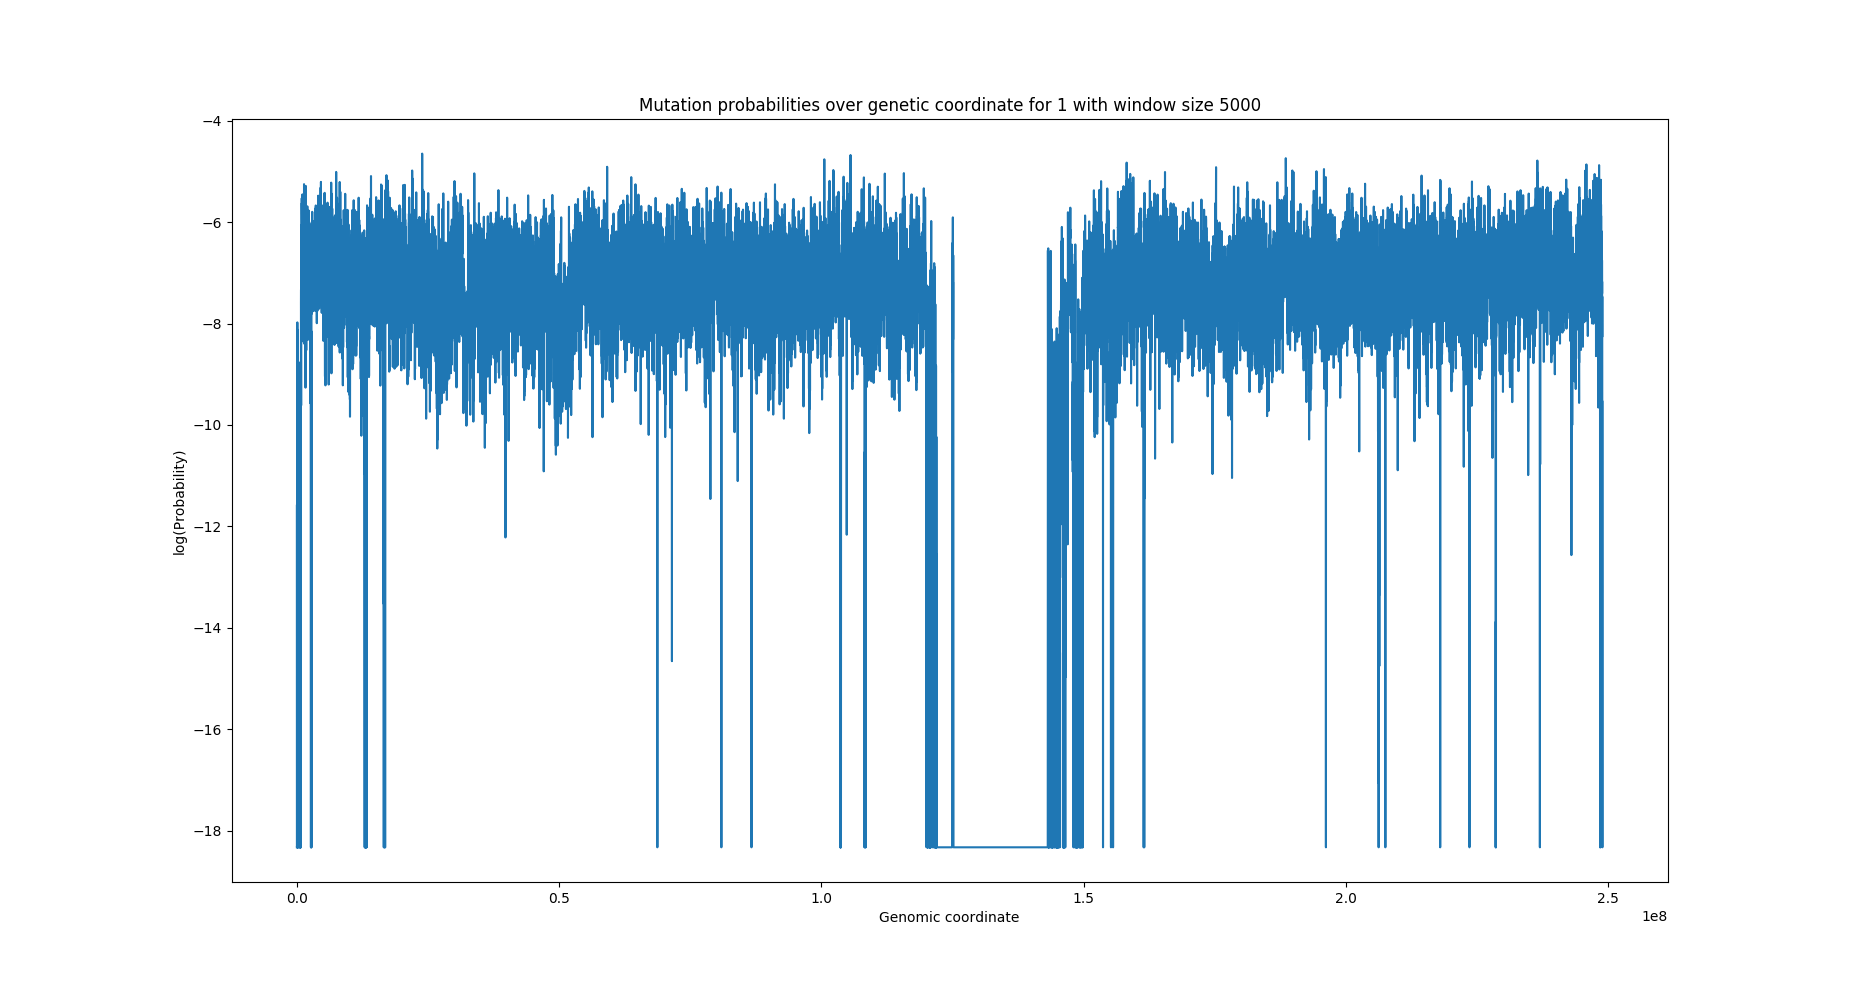
\includegraphics[width=6.0in]{testing/chr1_test/chr1_windowed_probabilities.png}}
\end{center}
   \caption{\small Windowed, location-contingent log probabilities of mutation. The regions in the center is adjacent to the centromere, for which there is no reference data due to the difficulty of sequencing the DNA. Therefore we ascribe very little probability (and thus very little confidence) to this region.}
\label{fig:windowprobs}
\end{figure}

For this work, we use publicly-available data from the 1000 Genomes Project \cite{5}. Variant Call Format (VCF) files were obtained from the official 1000 Genomes website for all chromosomes (1-22 and X) and parsed
using C++ and libvcf into HDF5 files containing the locations of mutations and the frequencies of base substitutions. Windowed average mutation probabilities were then computed for all chromosomes with $w = 5000$ (seen in Figure \cite{fig:windowprobs}),
which gave a good tradeoff between accuracy and speed, and output to a single combined VCF file. The chromosome 1 sequence from GRCh38 (GenBank accession CM000663.2) was downloaded, and an index for the sequence was built using bowtie2-index. The
sequence was then randomly mutated to produce artificial SNPs, and their positions were recorded. Then, artificial short reads of ~15X coverage were generated with errors from the mutated sequence using BBMap's randomreads
utility. Finally, the artificial reads were aligned to the reference chromosome 1 sequence, and variants were called using samtools mpileup (BCF format, with added DP and AD INFO tags) and filtered for positions
with one or more alternate calls. The resulting VCF file was used as input to BCaller along with the windowed mutation probability HDF5 file, and a minimum cutoff probability of 0.005 was applied. In Figure \ref{fig:outputprobs},
we display the output probabilities of the SNPs found in the artificial data. The probabilities of the true induced SNPs are much higher than the random mutations and give a more interpretable result than the unscaled scores
of many variant callers.

\begin{figure}[h]
\begin{center}
\fbox{ 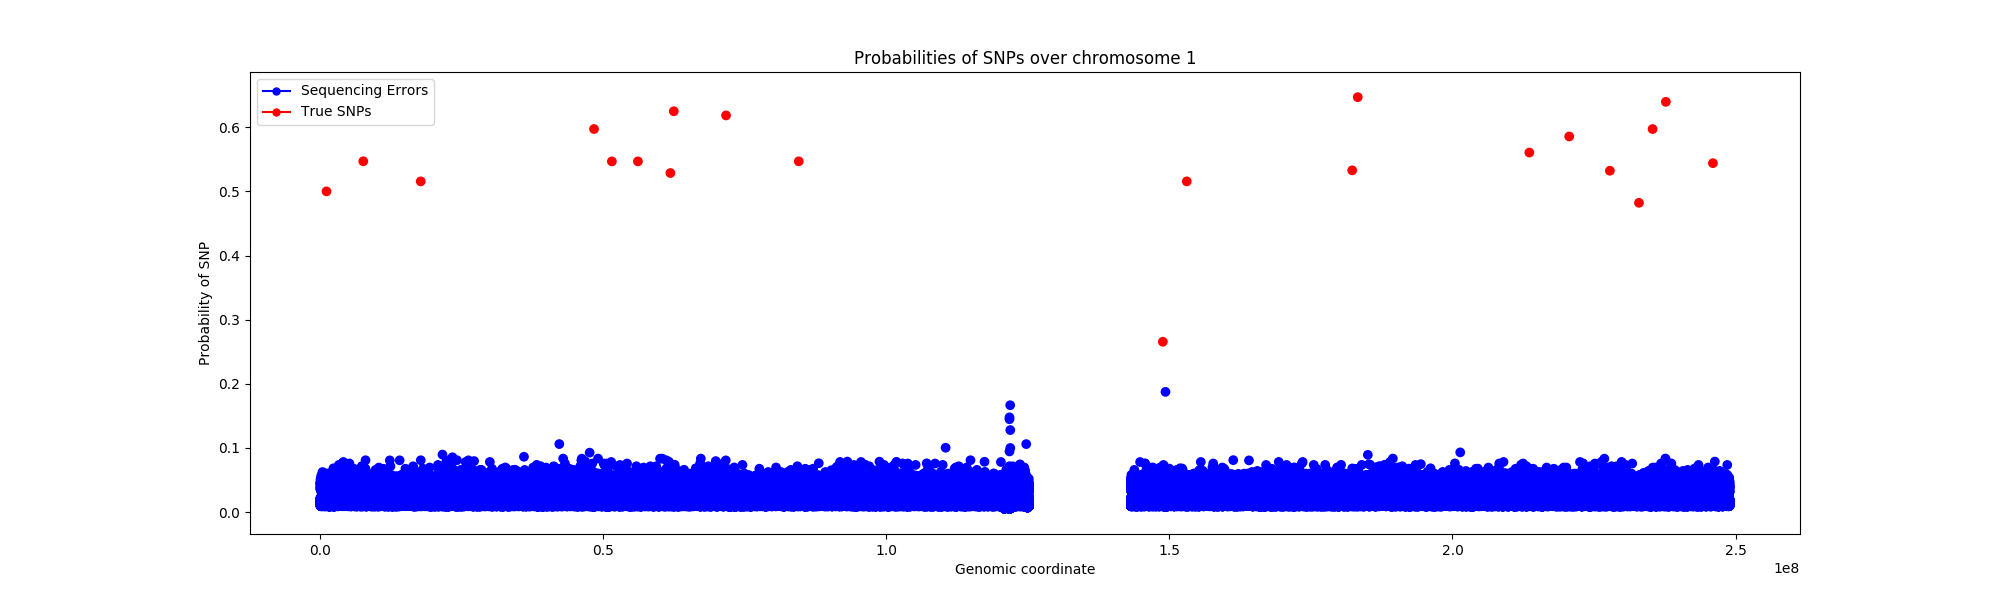
\includegraphics[width=6.0in]{testing/chr1_test/chr1_mutated_probabilities.png}}
\end{center}
   \caption{\small Probabilities of mutations from randomly generated reads. Blue points come from sequencing errors, red points are the true, introduced SNPs. The low score of one point comes from poor coverage of the random reads over that coordinate.}
\label{fig:outputprobs}
\end{figure}

\section{Further Work}

\par Although not done in this implementation, applying this work to heterozygous calls (e.g. in multiploid organisms such as \textit{H. sapiens}) would be simple; we can use the process of Bayesian model selection
to select a model corresponding to homozygous reference, heterozygous reference/alternate, heterozygous alternate, or homozygous alternate by simply computing the marginal likelihood of the model as follows:
\begin{equation}
\begin{aligned}
 p (M | D, X, B_1 \rightarrow B_2) = \int_\theta p(\theta | M, X, B_1 \rightarrow B_2) p(D | \theta, M, X, B_1 \rightarrow B_2) \ d\theta
\end{aligned}
\end{equation}
As we are using empirically-derived estimates for the distributions of $p(\theta | X, B_1 \rightarrow B_2)$, we can assume that $p(\theta | M, X, B_1 \rightarrow B_2) = p(\theta | X, B_1 \rightarrow B_2)$
(i.e. independence of the prior from the model).
$p(D | \theta, M, X, B_1 \rightarrow B_2)$ are modified according to expections of each model as follows:
\begin{itemize}
    \item For homozygous reference, we expect all calls to be reference.
    \item For heterozygous reference/alternate, we expect half of the calls to be reference, and half to be alternate.
    \item For heterozygous alternate, we expect half of the calls to be one alternate, and the other half to be a different alternate.
    \item For homozygous alternate, we expect all the calls to be alternate.
\end{itemize}
These assumptions are easy to encode using the generalization of this method. Instead of using a beta prior and a binomial likelihood, we extend into the multivariate case by placing a Dirichlet distribution on the
prior with $K = 4$ categories (one for each of the four cases) and place a categorical distribution on the likelihood. These are conjugate, and produce a Dirichlet-distributed posterior, giving similar speed and ease
of computation that is necessary for this task.

\par Another possible improvement to the caller could be to capture less granular information about the base substitutions; for example, instead of using single bases, base triplets could be captured to account
for interactions between various bases (this would capture some of complexity of CpG islands, transcript splice sites, promotor elements, etc.). In addition, gene location information could be used to account for
different mutation rates within genes and coding regions as opposed to intergenic regions (in fact, a smaller window could be used for coding regions to capture more granular information about conserved regions within genes).
In addition, other sources of genomic variant information can be used to further inform the location-contigent probabilties of mutation, including dbSNP and, with enough work, the Illumina SRA.

\section{Conclusion}
This work introduces a Baysian variant caller that uses publically
available data to inform variant calls. We focus on \textit{Homo sapiens} using single
nucleotide polymorphism (SNP) data from the 1000 Genomes Project to build mutation probability priors over the entire genome.
In addition, we show through artificial datasets that the method performs well in practice, even in the presence of sequencing errors.

{\small
\bibliographystyle{plain}
\bibliography{refs}{} % Create file refs.bib, and run bibtex.
}

\end{document}
